% confusion matrix
Confusion matrix is shown in Figure.\ref{fig:confusion_matrix} and some sample
training and testing images from the MIT-indoor67 dataset are shown in Figure.
\ref{fig:sample}

\begin{figure*}[ht]
  \centering
  \includegraphics[scale=0.16]{img/matrix.pdf}
  \centering
  \caption{From the confusion matrix of all 67 categories, we notice that several
pairs of categories are relatively easier to be confused and misclassified by the
SVMs with each other, such as bakery and deli, living room and bedroom as well as
bookstore and library.}
  \label{fig:confusion_matrix}
\end{figure*}

% sample image from dataset

\begin{figure*}[ht]
  \centering
  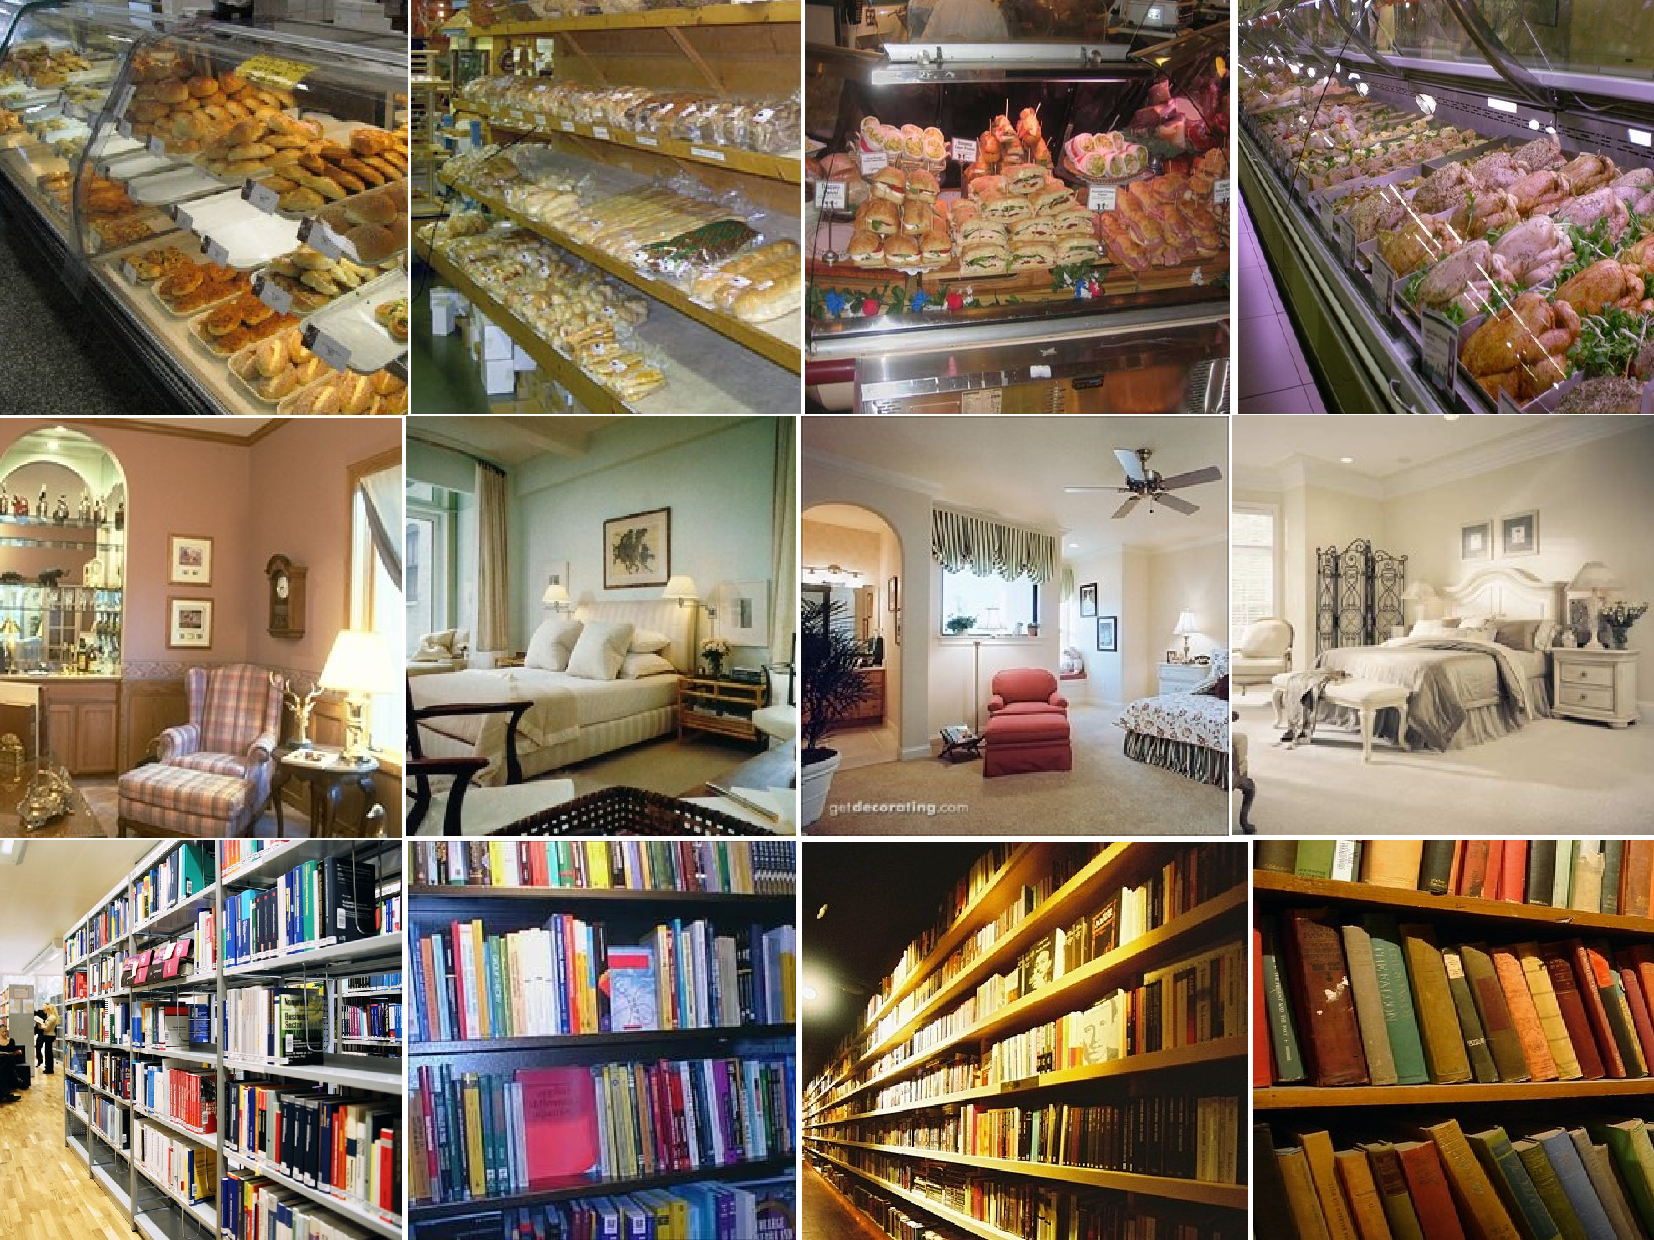
\includegraphics[scale=0.6]{img/dataset.pdf}
  \centering
  \caption{This figure contains some samples pairs from the MIT-indoor67 dataset.
For each line of image, left two are from the same category and right two are from
another. The first pair is bakery and deli which have very similar patterns of
listing of breads and sandwiches. The second pair is living rooms and bedrooms,
living room images may include some beds or beds-like sofas, which is almost
identical to the scenes in bedroom. It is extremely hard, even for human beings, to 
be able distinguish between library and bookstore.
the scene in bedrooms.}
  \label{fig:sample}
\end{figure*}